\quad U ovom poglavlju ulazimo dublje u pravila i funkcioniranje igre. Fokus će biti stavljen na neke pojedinosti koje su uzete u obzir prilikom implementacije ovog rada.\par 
Odmah se stavlja naglasak na to kako ovaj rad nije napravljen nad originalnom verzijom igre \textit{2048} već nad verzijom koju su razvili Krešo Orešković i Paulo Erak u sklopu projekta na Fakultetu elektrotehnike i računarstva (FER) pod mentorom Markom Đurasevićem. \par
U samom uvodu pokrili smo neke od najvažnijih elemenata i pravila igre koja su sadržana u obje verzije: \textit{Cilj igre je dobiti što veći rezultat koji je sam po sebi zbroj novostvorenih brojeva na ploči ispred nas. Imamo vrlo jednostavne poteze: pomicanje svih dijelova ploče lijevo, desno, gore ili dolje. Prilikom pomicanja, elementi koji su isti i susjedni, a nalaze se jedan drugome na putanji, spajaju se i time otvaraju prostor na ploči. Nakon svakog poteza se na nasumično otvoreno mjesto stavlja novi element.}\par
 Uzevši to u obzir, verzije igre nisu iste i neka pravila se razlikuju. Ta pravila bit će posebno naglašena u potpoglavlju \textit{Verzija igre korištena u radu}.\par 


\section{Originalna igra \textit{2048}}
Originalnu igru \textit{2048} napravio je talijanski programer, Gabriele Cirulli, koji je svoj rad \cite{2048og} postavio na internetsku uslugu za pohranu i upravljanje verzijama koda, GitHub.\par 
Igra se sastoji od nekoliko grafičkih elemenata: ploča (najčešća dimenzija je 4x4), kvadrati raznih boja koji sadrže brojeve (potencije broja 2) te se nalaze na ploči, brojači koji prikazuju trenutni i  najbolji rezultat i gumb za ponovo pokretanje igre.\newline
	\begin{figure}[h]
		\begin{subfigure}{0.5\textwidth}
			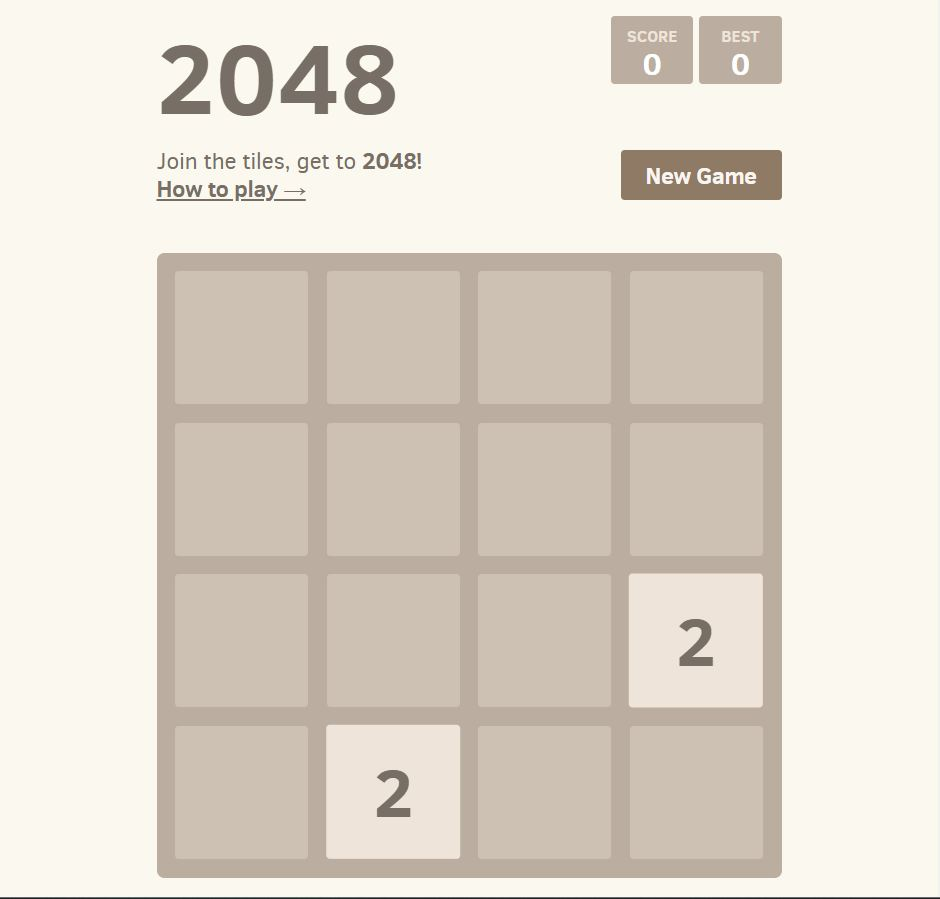
\includegraphics[width=0.9\linewidth, height=6cm]{originalni_2048} 
			\caption{Početno stanje}
		\end{subfigure}
		\begin{subfigure}{0.5\textwidth}
			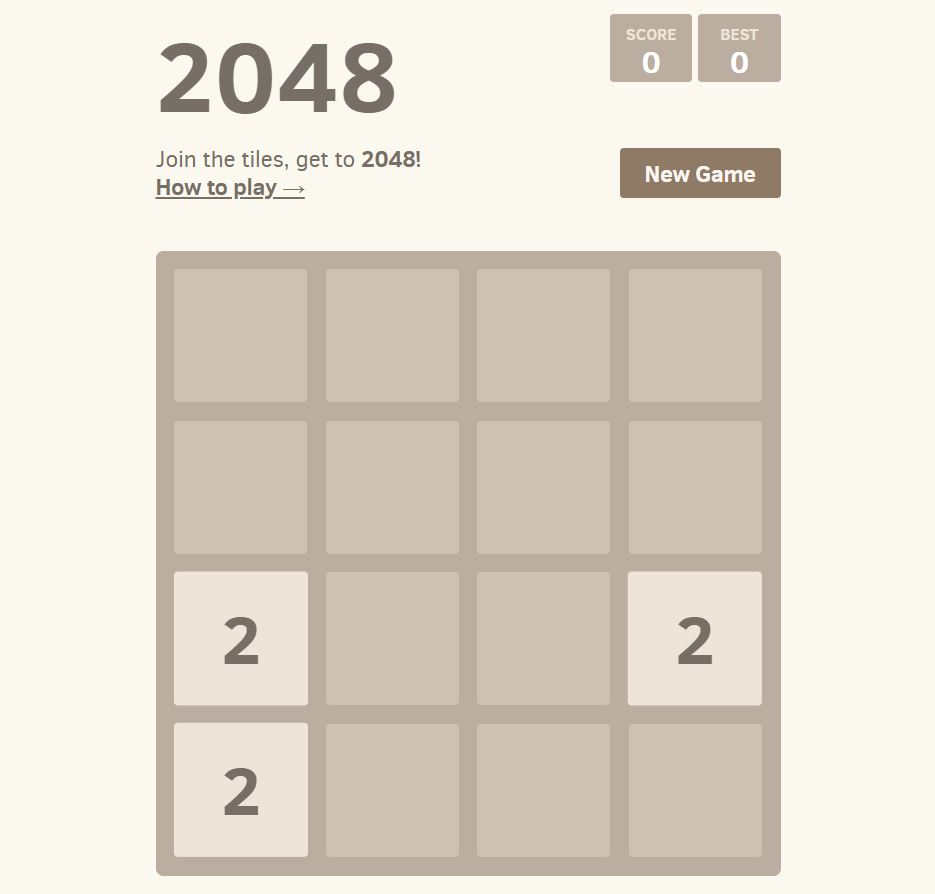
\includegraphics[width=0.9\linewidth, height=6cm]{originalni_2048_2}
			\caption{Potez u lijevo}
		\end{subfigure}
		
		\caption{Prikaz originalne igre \textit{2048} \cite{2048official}}
	\end{figure}
\newpage 
Potezima se svi postojeći elementi pomaknu u željenu stranu koliko i ako mogu, tj. ako im prazan prostor ili drugi elementi to dopuštaju. Primjer poteza može se vidjeti na slikama 2.1(a) i 2.1(b). Ako se dva ista kvadrata nađu jedan drugome na putanji spojit će se i proizvesti novi kvadrat s brojem jednakim zbroju brojeva u kvadratu. Spoj dva kvadrata s vrijednosti 2 prikazan je na slici 2.2.\newline
\begin{figure}[h]
	\centering
	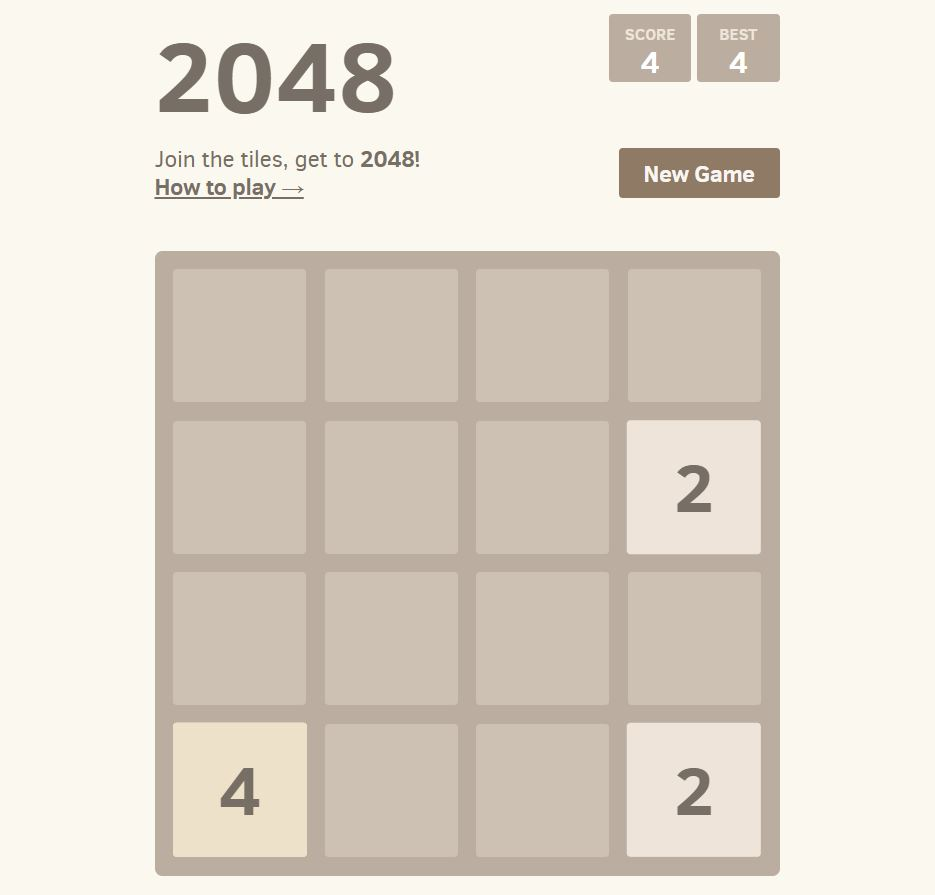
\includegraphics[width=0.5\linewidth]{originalni_2048_spajanje}
	\caption{Potez prema dolje, spajanje 2 i 2 \cite{2048official}}
\end{figure}
 \par
Potezi se ostvaruju pritiskom i puštanjem tipki strelica koje signaliziraju u kojem smjeru želimo pomaknuti sve elemente (gore,dolje,lijevo,desno). Potez se neće izvesti ako se njegovim izvođenjem neće izvesti nikakva promjena ploče, tj. nijedan element se neće pomaknuti zbog otpora drugog elementa ili ruba ploče. Držanjem strelice se postiže nekoliko rapidnih poteza u tom smjeru. Potezi prestaju otpuštanjem tipke ili ako se tim potezom neće pomaknuti niti jedan element. Kraj igre, Slika 2.3, nastaje ako imamo punu ploču i program prepozna da nijednim potezom nećemo postići promjenu rasporeda elemenata.\newline
\begin{figure}[h]
	\centering
	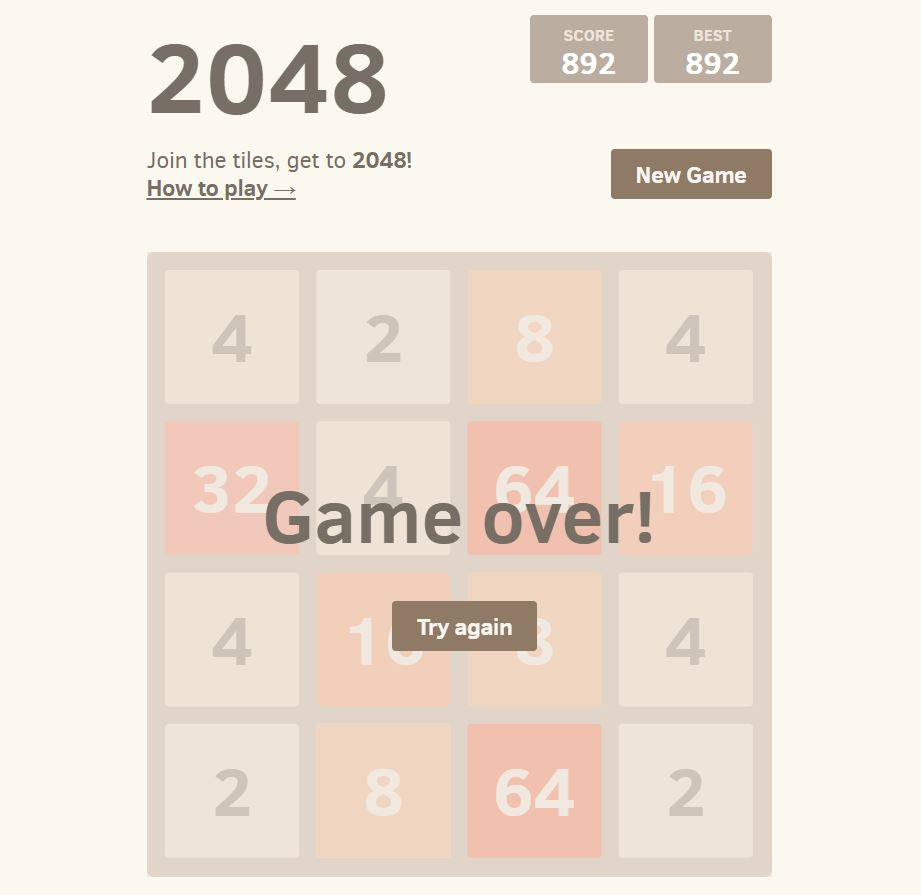
\includegraphics[width=0.5\linewidth]{originalni_2048_end}
	\caption{Kraj igre \cite{2048official}}
\end{figure}
\par
 Ako se dogodi da u jednom redu ili stupcu imamo poredak poput:
 \textbf{[2 2 4 8]} i napravimo potez u desno, dobit ćemo red: \textbf{[- 4 4 8]}. Dakle spajanje novih elemenata u potezu u kojem su napravljeni nije moguće. Ako imamo red oblika: \textbf{[2 2 4 4]}, potezom u desno dobivamo: \textbf{[- - 4 8]}. Višestruko spajanje elemenata je moguće te je omogućeno pomicanje u nove praznine u istom potezu.


\section{Verzija igre korištena u radu}
\quad Iako se ovaj rad referencira na originalnu igru, sam rad i njegova implementacija rađena je nad verzijom koja se po nekoliko elemenata razlikuje od originalne igre \textit{2048}.\par
Korištena verzija sadrži sljedeće grafičke elemente: ploča dimenzija 4x4, kvadrati raznih boja koji sadrže brojeve (potencije broja 2) te se nalaze na ploči, brojač koji prikazuju trenutni rezultat. Elementi se mogu vidjeti na slikama 2.4 i 2.5.
\par 
Prva bitna razlika u korištenoj verziji je ta da je rezultat zbroj brojeva na ploči, a ne zbroj brojeva u elementima koje je igrač dobio spajanjem. Iako je funkcionalnost donekle slična kao u početnoj verziji, vrijednost se više ne pripisuje igračevoj sposobnosti spajanja već se pripisuje količini i veličini brojeva na ploči.\newpage
\begin{figure}[h]
	\begin{subfigure}{0.5\textwidth}
		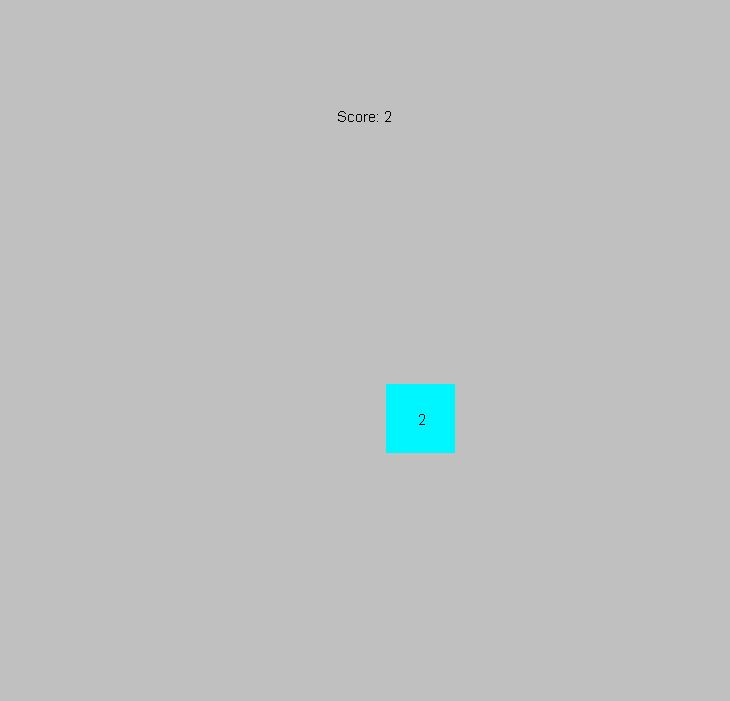
\includegraphics[width=0.9\linewidth, height=6cm]{nas_2048} 
		\caption{Početno stanje}
	\end{subfigure}
	\begin{subfigure}{0.5\textwidth}
		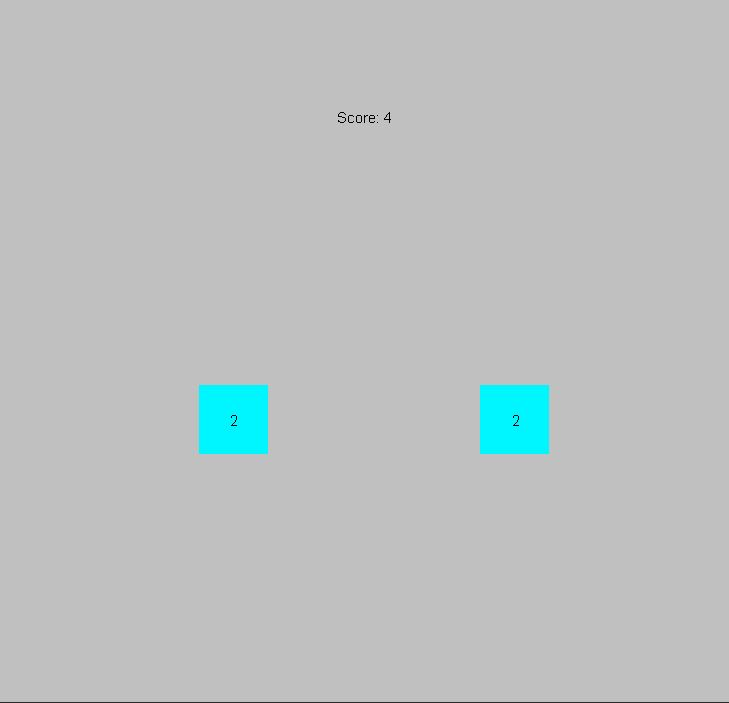
\includegraphics[width=0.9\linewidth, height=6cm]{nas_2048_2}
		\caption{Potez u lijevo}
	\end{subfigure}
	
	\caption{Prikaz korištene igre \textit{2048}}
\end{figure} 
Kretanja, ograničenja i spajanja elemenata na ploči slijede ista pravila kao i u originalnoj verziji igre.\newline
\begin{figure}[h]
	\centering
	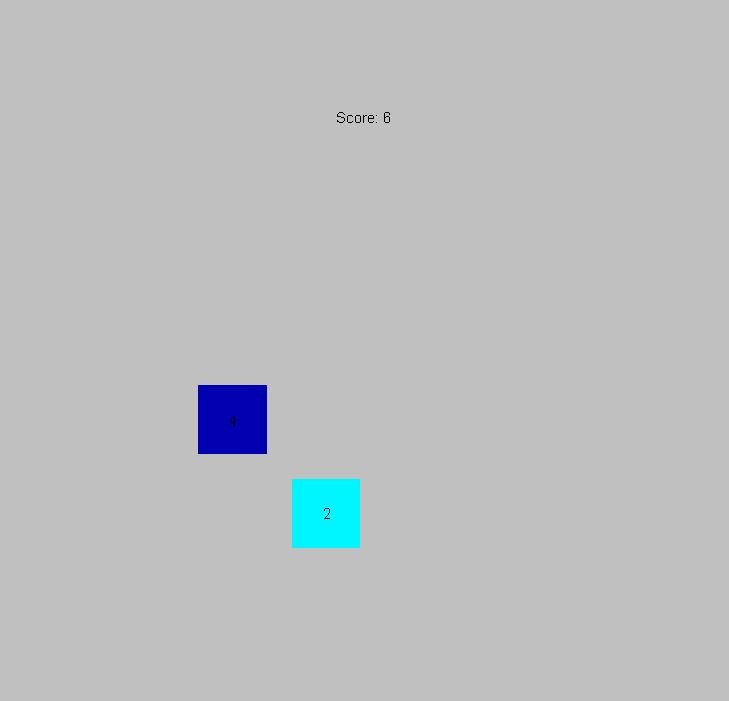
\includegraphics[width=0.5\linewidth]{nas_2048_spajanje}
	\caption{Potez prema lijevo, spajanje 2 i 2}
\end{figure}
\par
Potezi se ostvaruju pritiskom i \textbf{držanjem} tipki strelica koje signaliziraju u kojem smjeru želimo pomaknuti sve elemente. Ako se strelica ne drži do prestanka pomicanja svih elemenata postoji šansa da se igra počne nepredvidivo ponašati. Puštanje tipke strelice smatra se da je potez završio, a igra stvara novi element na nasumičnom slobodnom mjestu. Potezi će se izvesti čak iako se ne pomakne nijedan element. Kraj igre nastaje kad se pokuša dodati još jedan element na punu ploču.\par 
Ako se dogodi da u jednom redu ili stupcu imamo poredak poput:
\textbf{[2 2 4 8]} i napravimo potez u desno, dobit ćemo red: \textbf{[- - - 16]}. Dakle spajanje novih elemenata u potezu u kojem su napravljeni je moguće. Ako imamo red oblika: \textbf{[2 2 4 4]}, potezom u desno dobivamo: \textbf{[- - 4 8]}. Višestruko spajanje elemenata je moguće te je omogućeno pomicanje u nove praznine u istom potezu.\par 
Funkcioniranje verzije ovisi o grafičkom sučelju, a to stavlja veliko ograničenje na brzinu igranje igre. Potencijalna poboljšanja su smanjenje ovisnosti o grafičkom sučelju i promjena načina izvođenja poteza. To bi značilo da grafičko sučelje postane reprezentacija stanja koje je u pozadini, a ne ključni dio funkcioniranja igre, te da se potezi izvode na pritisak i puštanje tipki, a ne na držanje tipki.



